\subsection{The Jacobian criterion}

Let \(k\) be a ring, A a \(k\)-algebra, J an ideal of A, and \(\bar{d}:\mathrm{J / J^{2}}\to A /\mathrm{J}\otimes_{\mathrm{A}}\Omega_{k}(\mathrm{A})\) the canonical map. For each A/J-algebra R, we denote

\[
\bar {d} _ {\mathrm{R}}: \mathrm{R} \otimes_ {A / \mathrm{J}} \mathrm{J} / \mathrm{J} ^ {2} \longrightarrow \mathrm{R} \otimes_ {\mathrm{A}} \Omega_ {k} (\mathrm{A})
\]

the R-linear map deduced from \(\bar{d}\). If the k-algebra A/J is formally smooth, \(\bar{d}\) possesses an A-linear retraction (no. 2, remark 1) and \(\bar{d}_{R}\) has an R-linear retraction for every R.

More generally:

Lemma 3.--- Let K be an ideal of A containing J. Suppose there exists an integer m such that \(J \cap K^{m}\) is contained in JK (this condition is satisfied if A is Noetherian). If A/J is formally smooth over k for the K/J-adic topology, the map \(\bar{d}_{A/K}: A/K \otimes_{A/J} J/J^{2} \longrightarrow A/K \otimes_{A} \Omega_{k}(A)\) has an A-linear retraction.

Let C denote the \(k\) -algebra \(\mathrm{A} / (\mathrm{JK} + \mathrm{K}^m)\) ; the ideal \(\mathrm{N} = (\mathrm{J} + \mathrm{K}^m) / (\mathrm{JK} + \mathrm{K}^m)\) of C is square-zero, and the quotient ring C/N identifies with \(\mathrm{A} / (\mathrm{J} + \mathrm{K}^m)\) . Endow C and C/N with the discrete topology, and A/J with the K/J-adic topology. The canonical homomorphism \(\mathrm{A} / \mathrm{J} \to \mathrm{A} / (\mathrm{J} + \mathrm{K}^m)\) is continuous; it therefore has a lifting \(\varphi : \mathrm{A} / \mathrm{J} \to \mathrm{A} / (\mathrm{JK} + \mathrm{K}^m)\) .

The map \(a \mapsto a1_{\mathrm{C}} - \varphi(a1_{\mathrm{A/J}})\) from A to N is then a \(k\)-derivation ( \(n^{\circ} 1\) (prop. 1), hence can be written \(a \mapsto u(da)\) with \(u \in \mathrm{Hom}_{\mathrm{A}}(\Omega_k(\mathrm{A}), \mathrm{N})\). But the hypothesis \(\mathrm{J} \cap \mathrm{K}^m \subset \mathrm{JK}\) implies \(\mathrm{J} \cap (\mathrm{JK} + \mathrm{K}^m) = \mathrm{JK}\), so that the canonical map \(\psi: \mathrm{J/JK} \to \mathrm{N}\) is bijective; there therefore exists \(v \in \mathrm{Hom}_{\mathrm{A/K}}(\mathrm{A/K} \otimes_{\mathrm{A}} \Omega_k(\mathrm{A}), \mathrm{J/JK})\) such that, for a in A, we have \(a1_{\mathrm{C}} = \varphi(a1_{\mathrm{A/J}}) + \psi(v(1 \otimes da))\). Taking a in J, we see that \(v(1 \otimes da)\) is equal to the class of a in J/JK. Since \(\mathrm{A/K} \otimes_{\mathrm{A/J}} \mathrm{J/J}^2\) identifies with J/JK, v is the desired retraction.

The fact that the condition on K is satisfied when the algebra A is Noetherian follows from III, § 3, no. 1, cor. 2 of prop. 1.

Lemma 4.--- Suppose that A is formally smooth over k for the J-adic topology. For A/J to be formally smooth over k, it is necessary and sufficient that the canonical map \(\bar{d}\) has an A-linear retraction.

We already know that if A/J is formally smooth over k, the map \(\bar{d}\) admits an A-linear retraction (no. 2, remark 1). Conversely, suppose that \(\bar{d}\) possesses an A-linear retraction. Let \(\pi: A/J^{2} \to A/J\) be the canonical surjection; by prop. 2 of no. 1, there exists a ring homomorphism \(h: A/J \to A/J^{2}\) such that \(\pi \circ h = 1_{A/J}\). Let C be a k-algebra, N an ideal of C with square zero, and \(\rho: C \to C/N\) the canonical surjection; endow C and C/N with the discrete topology. Let \(u: A/J \to C/N\) be a continuous homomorphism of k-algebras. Since A is formally smooth over k for the J-adic topology, there exists a homomorphism of k-algebras \(v: A \to C\) making the diagram commutative

\pandocbounded{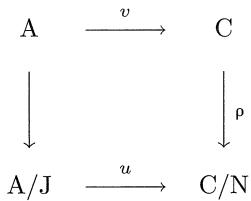
\includegraphics[keepaspectratio]{images/part001_bcdd9d30.jpg}}

where the vertical arrows represent the canonical surjections. We have \(v(\mathrm{J})\subset\mathrm{N}\), hence \(v(\mathrm{J}^{2})\subset\mathrm{N}^{2}=\{0\}\), and v defines, by passing to quotients, a homomorphism \(\bar{v}:\mathrm{A}/\mathrm{J}^{2}\to\mathrm{C}\) which satisfies \(\rho\circ\bar{v}=u\circ\pi\). Then \(\bar{v}\circ h\) is a lifting of u to C.

THEOREM 3.--- Let \(k\) be a ring, A a formally smooth \(k\)-algebra, and J a finitely generated ideal of A; set B=A/J.

\begin{enumerate}
\def\labelenumi{\alph{enumi})}
\tightlist
\item
  Let \(\mathfrak{p}\) be a prime ideal of B and let \(\mathfrak{q}\) be the (prime) ideal of A such that \(\mathfrak{p}=\mathfrak{q}/J\). The following conditions are equivalent:
\end{enumerate}

\begin{enumerate}
\def\labelenumi{(\roman{enumi})}
\item
  the k-algebra \(B_{\mathfrak{p}}\) is formally smooth;
\item
  there exists \(f\in B-\mathfrak{p}\) such that the k-algebra \(B_{f}\) is formally smooth;
\item
  the \(\kappa (\mathfrak{p})\)-linear map
\end{enumerate}

\[
\bar {d} _ {\kappa (\mathfrak {p})}: \kappa (\mathfrak {p}) \otimes_ {\mathrm{B}} \mathrm{J} / \mathrm{J} ^ {2} \rightarrow \kappa (\mathfrak {p}) \otimes_ {\mathrm{A}} \Omega_ {k} (\mathrm{A})
\]

is injective;

\begin{enumerate}
\def\labelenumi{(\roman{enumi})}
\setcounter{enumi}{3}
\tightlist
\item
  there exists an integer \(m \geqslant 0\) , elements \(f_{1}, \ldots, f_{m}\) of J, whose images \((f_{1})_{\mathfrak{q}}, \ldots, (f_{m})_{\mathfrak{q}}\) generate the ideal \(J_{\mathfrak{q}}\) , and k-derivations \(D_{1}, \ldots, D_{m}\) of A such that \(\det(\mathrm{D}_{j}(f_{i})) \not\in \mathfrak{q}\) .
\end{enumerate}

\begin{enumerate}
\def\labelenumi{\alph{enumi})}
\setcounter{enumi}{1}
\item
  The set of prime ideals p of B satisfying the equivalent conditions of (a) is open in Spec(B). For B to be formally smooth over k, it is necessary and sufficient that every prime (respectively maximal) ideal of B satisfy these conditions.
\item
  Suppose A is Noetherian. The conditions of (a) are also equivalent to:
\end{enumerate}

\begin{enumerate}
\def\labelenumi{(\alph{enumi})}
\setcounter{enumi}{21}
\tightlist
\item
  the k-algebra \(B_{\mathfrak{p}}\) is formally smooth for the topology \(\mathfrak{p}B_{\mathfrak{p}}\)-adic.
\end{enumerate}

Moreover, under the conditions of (iv), the ideal \(J_{\mathfrak{q}}\) is completely secant and the sequence \(((f_{1})_{\mathfrak{q}},\ldots,(f_{m})_{\mathfrak{q}})\) is completely secant for \(A_{\mathfrak{q}}\).

Set \(M = J/J^{2}\) and \(N = B \otimes_{A} \Omega_{k}(A)\) . The B-module \(M\) is of finite type, and the B-module \(N\) is projective ( \(n^{\circ} 5\) , cor. 3 of th. 2). For every multiplicative subset \(S\) of \(A\) , the \(k\) -algebra \(S^{-1}A\) is formally smooth ( \(n^{\circ} 2\) , prop. 4, a)). By lemma 4, conditions (i) and (ii) are therefore equivalent respectively to

(i') the map \(\bar{d}_{B_{\mathfrak{p}}}:M_{\mathfrak{p}}\longrightarrow N_{\mathfrak{p}}\) has a \(B_{\mathfrak{p}}\)-linear retraction;

(ii') there exists \(f \in \mathrm{B} - \mathfrak{p}\) such that the map \(\tilde{d}_{\mathrm{B}_f}: \mathrm{M}_f \to \mathrm{N}_f\) has a \(\mathrm{B}_f\)-linear retraction.

Prop. 9 of no. 8 applied to the ring B and to the homomorphism \(\bar{d}:M\to N\) implies the equivalence of conditions (i'), (ii'') and (iii), and also entails the assertions of (b) (using Lemma 4 again). Moreover, (iii) is equivalent to:

(iii') the map \(\kappa(\mathfrak{q})\otimes_{\mathrm{A}}\mathrm{J}\longrightarrow\kappa(\mathfrak{q})\otimes_{\mathrm{A}}\Omega_{k}(\mathrm{A})\) deduced from \(d:\mathrm{J}\to\Omega_{k}(\mathrm{A})\) is injective,

while (iv) can be written as:

(iv') there exists an integer \(m\geqslant 0\), elements \(f_{1},\ldots,f_{m}\) of J whose images generate the ideal \(J_{\mathfrak{q}}\) of \(A_{\mathfrak{q}}\), and elements \(y_{1},\ldots,y_{m}\) of \(\operatorname{Hom}_{\mathrm{A}}(\Omega_{k}(A),A)\) such that \(\det(\langle y_{j},df_{i}\rangle)\notin\mathfrak{q}\).

Since the \(\mathrm{A}\)-module \(\Omega_{k}(A)\) is projective (no. 5, cor. 3 of th. 2), prop. 9 of no. 8, applied to the ring A and to the homomorphism \(d:\mathrm{J}\to\Omega_{k}(A)\) provides the equivalence of (iii') and (iv').

Finally, suppose the ring A is Noetherian. It is clear that (i) implies (v). Under hypothesis (v), Lemma 3 implies that the map

\[
\bar {d} _ {\kappa (\mathfrak {q})}: \kappa (\mathfrak {q}) \otimes_ {\mathrm{B} _ {\mathfrak {p}}} \mathrm{J} _ {\mathfrak {q}} / \mathrm{J} _ {\mathfrak {q}} ^ {2} \longrightarrow \kappa (\mathfrak {q}) \otimes_ {\mathrm{A} _ {\mathfrak {q}}} \Omega_ {k} (\mathrm{A} _ {\mathfrak {q}})
\]

is injective, whence (iii).

Under the conditions of (iv), we have \(m=[\kappa(\mathfrak{q})\otimes_{\mathrm{A}}\mathrm{J}:\kappa(\mathfrak{q})]\) (no. 9, prop. 8). According to th. 2 of no. 5, the ideal \(J_{\mathfrak{q}}\) is completely secant, and the sequence \(((f_1)_{\mathfrak{q}},\ldots,(f_m)_{\mathfrak{q}})\) is completely secant for \(A_{\mathfrak{q}}\) (§ 1, no. 3, cor. 2 of th. 1). This proves c).

COROLLARY 1.--- Let \(k_{0}\) be a ring, \(k\) a Noetherian formally smooth \(k_{0}\)-algebra, and B a local \(k\)-algebra essentially of finite type. If the \(k_{0}\)-algebra B is formally smooth for the topology \(\mathfrak{m}_{\mathrm{B}}\)-adic, it is formally smooth.

There exists an integer \(n\geqslant 0\), a multiplicative subset S of \(k[\mathrm{T}_{1},\ldots,\mathrm{T}_{n}]\), and a surjective \(k\)-homomorphism \(\mathrm{S}^{-1}k[\mathrm{T}_{1},\ldots,\mathrm{T}_{n}]\to\mathrm{B}\). The algebra \(\mathrm{S}^{-1}k[\mathrm{T}_{1},\ldots,\mathrm{T}_{n}]\) is Noetherian and formally smooth over k (no. 3, Example 2 and no. 2, prop. 4, a)), hence over \(k_{0}\) (no. 2, prop. 3, a)). The corollary then follows from Theorem 3, c).

COROLLARY 2.--- Let \(k_{0}\) be a ring, \(k\) a Noetherian formally smooth \(k_{0}\)-algebra, and B a k-algebra essentially of finite type. The set U of prime ideals p of B such that the \(k_{0}\)-algebra \(B_{\mathfrak{p}}\) is formally smooth (for the discrete topology or the topology \(\mathfrak{p}B_{\mathfrak{p}}\)-adic) is open in Spec(B), and the following conditions are equivalent:

\begin{enumerate}
\def\labelenumi{(\roman{enumi})}
\item
  we have U = Spec(B);
\item
  U contains all the maximal ideals of B;
\item
  the \(k_{0}\)-algebra B is formally smooth.
\end{enumerate}

This follows as before from Theorem 3.

Note 1.--- Corollaries 1 and 2 apply in particular when \(k_{0}\) is a field and we are in one of the following two cases:

\begin{enumerate}
\def\labelenumi{\alph{enumi})}
\item
  B is an algebra essentially of finite type over a separable extension of \(k_{0}\) (th. 1 of no. 3);
\item
  B is a \(k_{0}\)-complete Noetherian local algebra whose residue field \(\kappa_{B}\) is a separable extension of \(k_{0}\) (in this case we take for k an algebra of formal power series over \(\kappa_{B}\) of which B is a quotient (no. 3 and IX, § 3, no. 3)).
\end{enumerate}

In each of these cases, it follows from Cor. 2, taking into account Prop. 8 of No. 7 and Prop. 6, b) of § 6, No. 4, that the \(k_0\)-algebra B is formally smooth if and only if it is absolutely regular.

COROLLARY 3 (Zariski). Let \(k\) be a field, A a \(k\)-local regular algebra, and J an ideal of A distinct from A. We assume that the \(k\)-algebra A is essentially of finite type or complete. For the local ring A/J to be regular, it is necessary and sufficient that there exists an integer \(m \geqslant 0\) , elements \(f_1, \ldots, f_m\) of J generating J and derivations D \(_1, \ldots, D_m\) of A such that det(D \(_j(f_i)\) ) \(\not\in \mathfrak{m}_{\mathrm{A}}\). The elements (f \(_1, \ldots, f_m\) ) then form part of a coordinate system of A and the ideal J is prime.

Let \(k_0\) be the prime subfield of \(k\). The \(k_0\)-algebra A is absolutely regular (§ 6, no. 4, Example 1), hence formally smooth (Remark 1 above). For the same reasons, saying that A/J is regular is equivalent to saying that it is a \(k_0\)-algebra formally smooth. The first assertion therefore follows from Theorem 3, which also implies that the sequence \((f_1,\ldots,f_m)\) is completely secant for A. One then applies Proposition 2 of VIII, § 5, no. 3.

Remark 2.--- Under the hypotheses of Cor. 3, the A-module \(\Omega(A)\) is projective (no. 5, Cor. 3 of Theorem 2), hence free; every derivation of A into \(\kappa_{A}\) therefore lifts to a derivation of A. The condition of the statement can thus be expressed as follows: there exists a generating system \((f_{1},\ldots,f_{m})\) of J and derivations \(D_{1},\ldots,D_{m}\) of A into \(\kappa_{A}\) , such that \(\det(D_{j}(f_{i}))\neq0\).

COROLLARY 4 (Zariski).--- Let k be a field and A a k-algebra essentially of finite type or a complete Noetherian local ring. The set of prime ideals p of A such that the local ring A \(_{p}\) is regular is open in Spec(A).

It suffices to apply Remark 1, taking for \(k_0\) the prime subfield of \(k\).

